% Session 1 -- the mean-field self-consistency loop.
% Placement: sec. "Worked example 1", at the "more rigorously, mean-field theory is a
% variational search..." paragraph.
% Rendered by figures/blender/s01f05_selfconsistency.py, labels in figures/overlays/s01f05_selfconsistency.tex.
\begin{aqmfigure}{fig:s01:mfloop}{The mean-field self-consistency loop. We guess the bilinear
expectation values, build the single-particle Hamiltonian that they give, and diagonalize it. Then
we compute the new expectation values and repeat until they do not change anymore. The four stations
are one pass of the loop, computed for the charge density wave of (1.6) on a periodic chain of four
sites with $V=3t$. The guessed charges $0.6$ and $0.4$, drawn as columns, raise the onsite energy of
the neighboring sites, so the sites of the mean-field Hamiltonian stand at two heights. Filling its
two lowest levels gives the new charges $0.82$ and $0.18$, which are not the guess, so the loop goes
round again. The three worked examples of this session and every notebook box in this chapter use
this same loop.}
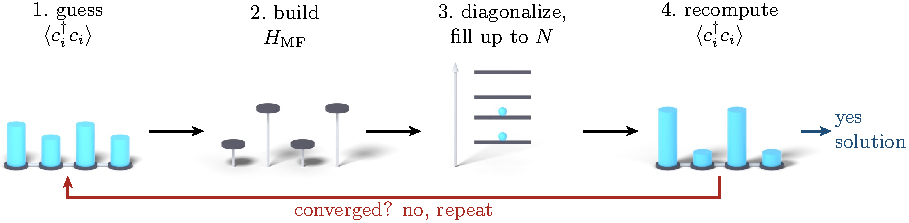
\includegraphics{figures/pdf/s01f05_selfconsistency.pdf}
\end{aqmfigure}
